\chapter{Nonparametric Machine Learning Methods in Recommender Systems}
\label{chap:ml}

Here we will introduce some famous machine learning (ML) methods, and apply
them to recomender systems (RS).  In fact, many of the complex RS
methods used in industry are hybrid, typically combining an ML method
such as neural networks with matrix factorization; see for instance an
article on the hybrid system used as Netflix.\footnote{https://ojs.aaai.org/index.php/aimagazine/article/view/18140}

In contrast to our previous methods for estimation a regression
function---the linear and logistic models, polynomial models, and LASSO
and ridge, the methods used in this chapter are all
\textit{nonparametric}, meaning that there is no ``$\beta$,'' no
parameter vectors specifying the structure of the regression
function.\footnote{A partial exception will be SVM, where a `$\beta$''
is estimated that, while not the regression function, is related to that
function.}

\section{K-Nearest Neighbor}

We've seen this method, extremely simple.  Say we wish to predict the
weight of a person 70 inches tall and 25 years old, given
data on people with known height, weight and age.  We find $k$
people in our data whose height and age are near 70 and 25, and average
their weights.  This will be the predicted weight for the new person.
The value $k$ is a hyperparameter.

While k-NN is very useful in RS, its application is a bit less
straightforward than in that height-weight-age example.  Let's see why.

Recall that in Section \ref{lincollab}, we found that predicting rating
from just user and item IDs did not work well.  The IDs needed to be
converted to dummy variables, resulting in a large number of features $p$
and possible overfitting.  If we instead predicted from the embeddings
user and item mean ratings, we get better accuracy.

The same large-$p$ problem occurs if we try to use k-NN to predict
rating from user and item IDs.  Again, using the embeddings is a better
bet:

\begin{lstlisting}
> qeKNN(ml100kpluscovs[,c('rating','userMean','itemMean')],'rating')$testAcc
holdout set has  1000 rows
[1] 0.75036
\end{lstlisting}

\subsection{K-NN in RS Has Special Issues}

There are also problems with using k-NN just on the IDs.  Think of what
happens in the process of finding neighbors.  To predict the rating
that, say, User 12 would give Item 88, we would first look at that 
user's vector of dummy variables (1 for rated, 0 for not).  The closest
rows to this user will have rated mostly the same items as this user.
That may be worth something, but it would be better if we could compare
the ratings themselves:  Among the items that User 12 has rated, which
rows (a) have ratings for the same items, and (b) having ratings similar
to those of User 12 for those items?

\subsection{Implementation in rectools}

The relevant functions are \textbf{formUserData()} and
\textbf{predict.usrData()}.  True to its name, the latter does do
prediction.  The former works on the training set, but in a very
different way from what we've seen so far.

For instance, our first step with the MovieLens data would be:

\begin{lstlisting}a
> udata <- formUserData(ml100[,-4])
> class(udata)
[1] "usrData"
> udata[[88]]
$userID
[1] "88"

$itms
 [1]  750  302  321  881  301  315  261  690  904  886  308  311  300 1191  319
[16]  313  880  898  354  286  326

$ratings
 750  302  321  881  301  315  261  690  904  886  308  311  300 1191  319  313 
   2    3    1    5    4    4    5    4    5    5    4    5    3    5    3    3 
 880  898  354  286  326 
   3    4    5    5    5 

attr(,"class")
[1] "usrDatum"
\end{lstlisting}

So, \textbf{formUserData()} returns an object of class
\textbf{'usrData'}, which is an R list.  Each element of the list
represents the data on one user; we see that user 88, for instance, has
rated movies 750, 302, 321 and so on, and with ratings 2, 3, 1 etc.
 
This allows an efficient structure for searching for neighbors of a user
for whom we wish to form a prediction.  The latter operation is then
performed using the second function:

\begin{lstlisting}
# predict the rating that User 12 would give to Item 15, using k = 8
> predict.usrData(udata,udata[[12]],25,8)
[1] 3.625
\end{lstlisting}

\subsection{Assesment of Predictive Ability}

Note that, unlike the case for other methods, we do not need to split
into training and test sets.  Recall that such a split is needed in
general to avoid having the same data used for both model fitting and
prediction.  With k-NN, though, as long as we don't treat a data point
as its own ``neighbor,'' it is fine.

Here is an assessment of k-NN for the MovieLens data:

\begin{lstlisting}

> predOneRow
function(rw)
{
   user <- rw[1]
   item <- rw[2]
   predict.usrData(udata,udata[[user]],item,5)
}
> preds <- apply(mvl[,-3],1,predOneRow)
> mean(abs(mvl[,3] - preds))
[1] 0.5706778

\end{lstlisting}


\subsection{Not Really a Distance}

In many ML algorithms, the ``distance'' computed between two objects 
does not use the ordinary Euclidean metric.  In fact, it's not a metric,
but rather a ``similarity.''

The similarity between two rows $u$ and $v$ in the ratings matrix
is defined by

\begin{equation}
\frac{u'v}{||u||_2 ~ ||v||_2}
\end{equation}

In two or three dimensions, this actually is the cosine between the two
vectors.  Note too that if $u$ and $v$ were centered, i.e. had their
means subtracted, this would be the definition of correlation.  In other
words, two users are considered similar to each other if their ratings
are highly correlated.  That makes this similar measure intuitively
reasonable, though only if they had similar means to begin with.  If,
say, $v = 2u$, their similarity would have the maximum value, +1, yet we
would want to scale $v$ down if we wish to predict $u$ from it.

\section{Decision Trees and Random Forests}

\textit{A decision tree} is a set of prediction rules formed in a flow
chart.  (Example below.)  The idea was developed by many, but first
became popular with the algorithm Classicification and Regression Trees
(CART), by famous statistician Leo Breiman, Jerry Friedman, Richard
Olshen and Chuck Stone.  (Stone's theoretical work on k-NN also helped
to popularize that method.)

Credit for the invention of random forests is generally given to
Breiman, but actually the earliest proposal seems to have been by Tin
Kam Ho.  She called the method \textit{random decision forests}.  What
is all this about?

We first must discuss individual ``trees

\subsection{Decision Trees}

Many have worked in the area of decision trees, which are essentially
flow charts.  As an example, here is an example from the \textbf{party}
package,\footnote{A pun on the word ``partitioning''; a tree
partitions the dataset.} run on the dataset \textbf{airquality} built in
to R.

\begin{lstlisting}
> head(airquality)
  Ozone Solar.R Wind Temp Month Day
1    41     190  7.4   67     5   1
2    36     118  8.0   72     5   2
3    12     149 12.6   74     5   3
4    18     313 11.5   62     5   4
5    NA      NA 14.3   56     5   5
6    28      NA 14.9   66     5   6
\end{lstlisting}

We are predicting \textbf{Ozone}.  Here is the tree that is produced
(picture from the \textbf{party} package's \textbf{plot()} function):

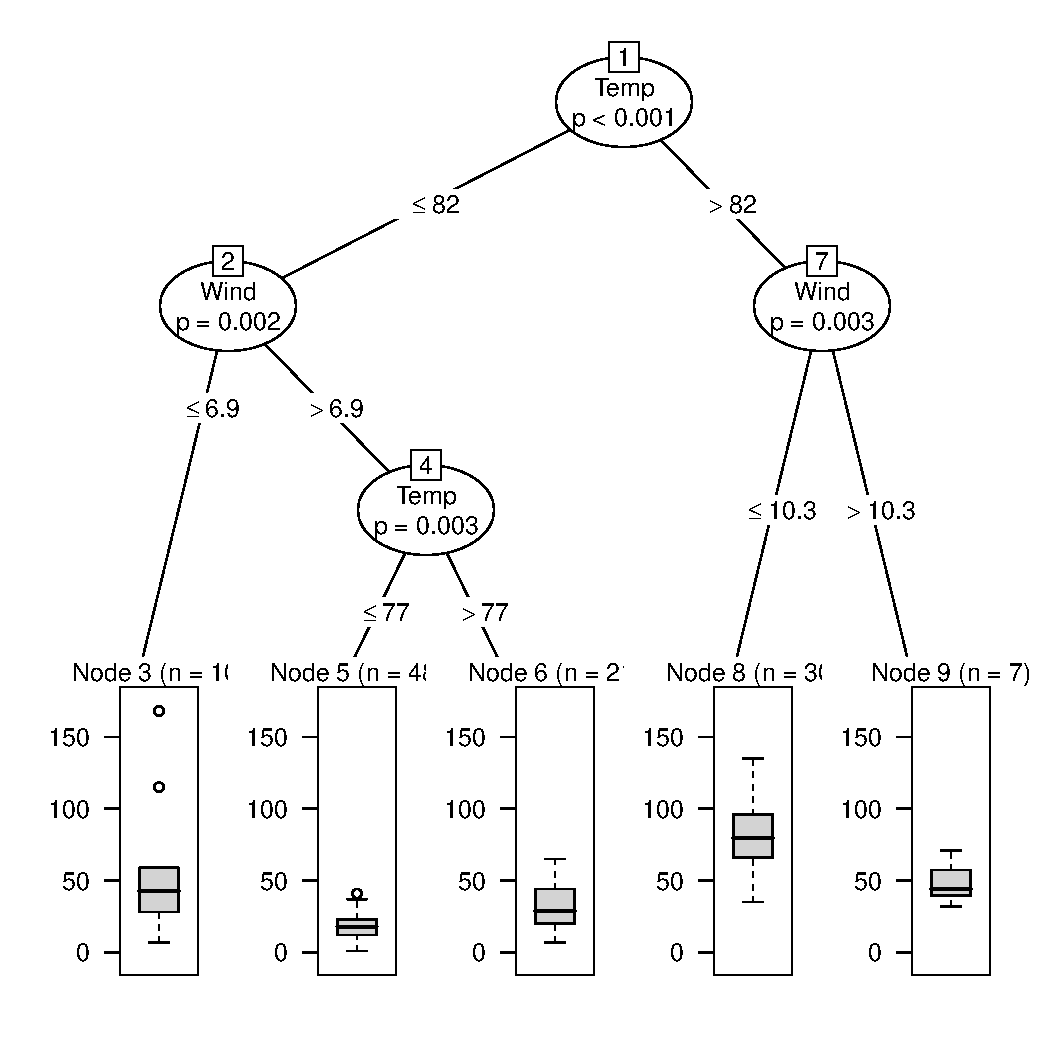
\includegraphics[width=4.5in]{AirQCTree.pdf}

To predict \textbf{Ozone} level on a particular day, we start at the
root of the tree, looking at \textbf{Temp}.  If it is less than 82, we
next go left, otherwise to the right.  In the latter case, we next look
at \textbf{Wind}.  Say it's greater than 10.3.  Then we end up in Node
8, predicting \textbf{Ozone} to be about 50.  More precise predictions
are also provided (not shown in the plot).

The final predicted value for a new case is determined as follows:  We
first note that leaf nodes that each of the data points in the training set
fall into.  Then for a new case, its predicted value is the average of
all the \textbf{Ozone} values for the training set data points in the
node in which the new case falls.

There are various hyperparameters.  For instance, note that here Node 6
has only 2 training set data points.  Taking an average of a sample of 2
numbers is not going to be very accurate.  So the software gives the
user the option of specifying a minimum number of points in each node.
If we were to increase that here, we would probably have fewer levels in
the tree.  We can also specify that number.  Of course, this dataset is
very small, only 153 rows, so there is not much room for trying
different hyperparameter values.

\subsection{Splitting Criteria}

So, how is the tree derived?  We start with all the training data in the
root node.  We then decide whether to split the node, using our first
feature, \textbf{Temp} in the above example.  If we do split it, we now
have three nodes, and decide whether to split them.  This is then
continued recursively until no more splits are done.

What criteria should we use to decide whether to split a node?
Splitting criteria tend to be complex, and different implementations of
decision trees and random forests use different criteria.

In the \textbf{party} package, a hypothesis testing approach is used.
It considers all possible split points, such as 82 in the example.  For
each split point, we tentatively split into two groups,  We then do a
hypothesis test for mean ``Y'' (ozone here) being the same in the two
groups.  We look at the smallest p-value coming from the various splits;
if it is below our specified threshold (another hyperparameter), we do
that split.  If no p-value is below our threshold, we do not split.
So, in the picture above, Nodes 8 and 9 were not split, and became leaf
nodes.

\subsection{Sets of Many Trees}

\noindent
\begin{quote}
{\it
For want of a nail, a horse was lost \\
For want of a horse, the battle was lost \\
For want of the battle, the war was lost
} --- old proverb
\end{quote}

In the tree shown above, look at the output of Node 7.  Depending on
whether \textbf{Wind} is below or above 10.3, we get very different
predictions.  If wind speed is, say, 10.28, very close to the threshold,
we may be wary, especially since the wind speed itself may not be
measured very accurately.

To overcome problems arising from this discrete nature of decision
trees, we generate many of them, randomizing the order in which we make
nodes from the features, thus creating \textit{random forests}.

To predict a new case, we run it through each tree, thus generating a
predicting value from each tree.  Those values are then averaged to
determine the final predicted \textbf{Ozone} level.

The number of trees to generate is---you guessed it!--yet another
hyperparameter.

\subsection{Example:  Baseball Data}

Recall our data on major league baseball players:

\begin{lstlisting}
> library(regtools)
> data(mlb)
> mlb <- mlb[,3:6]
> head(mlb)
        Position Height Weight   Age
1        Catcher     74    180 22.99
2        Catcher     74    215 34.69
3        Catcher     72    210 30.78
4  First_Baseman     72    210 35.43
5  First_Baseman     73    188 35.71
6 Second_Baseman     69    176 29.39
\end{lstlisting}

Let's try predicting \textbf{Weight}:

\begin{lstlisting} 
> qeRF(mlb,'Weight')$testAcc
[1] 14.43367
\end{lstlisting}

On average, our prediction is off by about 14 pounds, about the same
accuracy as we got with a linear model in Section \ref{firstqelin}.
Let's try a minimum node size of 25, instead of the default 10:

\begin{lstlisting}
> qeRF(mlb,'Weight',minNodeSize=25)$testAcc
[1] 13.10866
\end{lstlisting}

Seems better, though we should use \textbf{replicMeans()}, try other
hyperparameter combinations, and so on.

\subsection{Example:  MovieLens}

In collaborative filtering contexts, most ML methods encounter the 
problem cited earlier if we predict rating from user and item IDs---too 
many dummy variables.  But once again, we can use embeddings.  We'll try
\textbf{grf}, a faster, more advanced implementation:

\begin{lstlisting}
> mluimeans <- ml100kpluscovs[,c('rating','userMean','itemMean')]
> qeRFgrf(mluimeans,'rating')$testAcc
[1] 0.7319664
\end{lstlisting}

This is about the same as we obtained with a linear model, not as good
as k-NN, though again there are hyperparameters to vary.

\section{Gradient Boosting:  Repeatedly Tweaking a Tree}

\textit{Boosting} methods, of which \textit{gradient boosting} is one
type, are sometimes described as ``Making a strong learner as the
sum of weak learners.''  I am not a fan of that interpretation, but it
will become clear as we go through the details.

\subsection{Basic Idea}

The idea of \textit{gradient boosting} is extremely simple: 

\begin{itemize}

\item [(a)]  Fit a tree to the data.

\item [(b)]  Find the prediction errors, the \textit{residuals,}
for that tree (on the same data,).

\item [(c)]  Fit a tree to the residuals, producing \textit{new}
residuals.

\item [(d)]  Go to step (b).

\end{itemize} 

One keeps up this process until one acquires a desired number of trees
(a hyperparameter).  

To predict a new case, use its features to get a predicted value for
each tree.  Then since the first tree was fitted to the $Y_i$, and the
others were fitted to the residuals, the residuals of residuals and so
on, then \textit{our overall predicted value for the new case is the sum
of the predicted values from the individual trees}.

% \begin{itemize}
% 
% \item [1.]  Using our features, fit a tree to our $Y$ data,
% $Y_1, Y_2,...,Y_n$.  Name this tree $T_0$, and 
% let $Y_i^{0}$ denote the values predicted by this 
% tree,  $i = 1,2,...,n$.
% 
% \item [2.]  Look at the \textit{residuals}, the prediction errors,
% 
% \begin{equation}
% R_i^{(0)}
% \end{equation}
% 
% \end{itemize} 

\subsection{Role of the Gradient}

At each step, we try to fit the optimal tree, minimizing Mean
Squared Prediction Error.  To do so, we could set the derivative (in $p$ 
dimensions, the \textit{gradient}), to 0.  But with the MSPE objective
function, the partial derivative with respect to data point $i$
is essentially the residual $i$.  So, in Step (c) above, we are
essentially fit a tree to the gradient values at each data point.

\subsection{The Learning Rate}

One typically sets a learning rate $\alpha$ (another hyperparameter).
So, each time a new tree is generated, instead of adding its residuals
to our running total, we only add $\alpha$ times those residuals.  

Note that this has the effect that the residuals in tree $i$ will have
an impact of only $\alpha^i$ of the first set of residuals.  This sets
up convergence of the overall tree.  The larger $\alpha$ is, the faster
the convergence---but at a risk of converging to the wrong value, a
local rather than global minimum.  Of course, this is the usual tradeoff
of learning rates.

\subsection{Variants}

The above description is for tree-based gradient boosting, with
MSPE is the loss function.  Of course there are many other
possibilities, though this one is probably the most common..

\subsection{Rec Sys Example}

Gradient boosting gives us similar values to the other (non-k-NN)
methods on the MovieLens data:

\begin{lstlisting}
> qeGBoost(ml100kpluscovs[,c('rating','userMean','itemMean')],'rating')$testAcc
[1] 0.7389659
\end{lstlisting}

\section{Support Vector Machines}

SVM is used primarily for the cases of binary or categorical $Y$.
Consider the binary case, $Y = 1,0$ (coding Has Disease, Does Not have
Disease).  

\subsection{Overview}

Here is a summary, for given training data, $p$ predictor
variables/features (e.g.\  $p = 2$ with features Blood Pressure and
Glucose):

\begin{itemize}

\item We try to find a straight line ($p = 2$ case), a plane ($p = 3$)
or a hyperplane ($p > 3$) that fully separates our training points
having $Y = 1$ from those having $Y = 0$.  This can be shown to be
equivalent to minimizing a sum of a loss function (more complicated than
squared-error loss, not shown here).

\item If we find such a line/plane/hyperplane, then for any new case, we
simply determine which side of the line/plane/hyperplane the new point
falls on, and predict the $Y$ for the new point accordingly

\item If we can't find a fully separating line/plane/hyperplane, we do
one or both of the following:

   \begin{itemize}

   \item Apply a tranformation to the features, e.g.\ running them
   through a polynomial, in the hope that the tranformed data can be
   cleanly separated by $Y$ class, with some line/plane/hyperplane.  The
   degree of the polynomial is a hyperparameter.

   \item In minimizing the summed loss, allow some exceptions to cleanly
   separating the two classes, with each exceptional point penalizing us
   with a cost $C$, again a hyperparameter.
   
   \end{itemize} 

\end{itemize} 

If $Y$ has more than two categories, we use the One vs.\ All or All vs.\
All method.

\subsection{Example:  Anderson Iris Data}

This is a very famous dataset, built into R and used as an example in
numerous textbooks, was compiled by Edgar Anderson and later popularized
by Sir Ronald Fisher, a pioneering statistician.\footnote{A few years
ago, Fisher was ``canceled'' by some social activists, who wanted other
data to be used an example, rather than use his name.  But the data
should be named after Anderson anwyay.} There are three classes,
\textit{setosa}, \textit{versicolor} and \textit{virginica}.  It turns
out that the setosa data points are linearly separable from the other
two classes, so this is a good place to start.  Thus, our two classes
will be setosa and non-setosa.  As before, in order to graph things in
two dimensions, let's use only two of the features, sepal width and
petal length:

Let's take a look:

\begin{lstlisting}
> i2 <- iris[,c(2,3,5)]
> i2[,3] <- as.integer(i2[,3] == 'setosa')
> head(i2)
  Sepal.Width Petal.Length Species
1         3.5          1.4       1
2         3.0          1.4       1
3         3.2          1.3       1
4         3.1          1.5       1
5         3.6          1.4       1
6         3.9          1.7       1
> plot(i2[,1:2],pch=3*i2[,3],xlim=c(0,7),ylim=c(0,7))
\end{lstlisting}

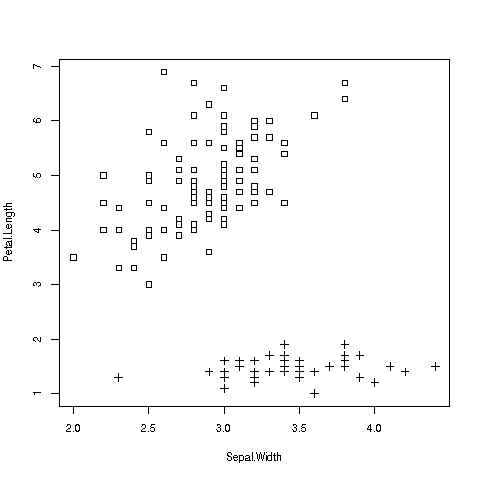
\includegraphics[width=3in]{IrisOrigNew.png}

Clearly the data are linearly separable --- we can draw a straight line
completely separating the setosas (pluses) from the non-setosas
(squares).  In fact, we can draw lots and lots of such lines.

Which line should we use?  One can show that if we draw the convex hull
of the $Y = 1$ data, and one for the $Y = 0$ data, minimal loss line is
the perpendicular bisector between the closest points of the two sets.

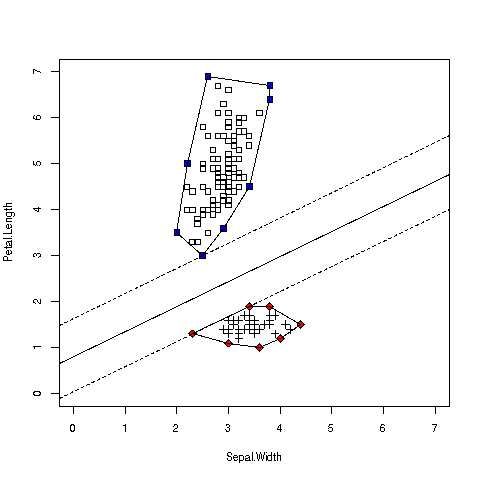
\includegraphics[width=3in]{IrisConvNew.png}

The actual computation for the separating line/plane/hyperplane does not
use this convex hull property, but it gives us an intutive view.

\subsection{Example:  House Voting Data}

\begin{lstlisting}

>  hv <- getHouseVoting()
>  hv <- hv[,-17]
>  hvsyn <- toUserItemRatings(hv)
>  ums <- tapply(hvsyn$ratings,hvsyn$userID,mean)
>  hvsyn$uMean <- ums[hvsyn$userID]
>  ims <- tapply(hvsyn$ratings,hvsyn$itemID,mean)
>  hvsyn$iMean <- ims[hvsyn$itemID]
>  hvsyn$ratings <- as.factor(hvsyn$ratings)
>  z <- qeSVM(hvsyn[,3:5],'ratings')
> z$testAcc
[1] 0.3963415
> z$baseAcc
[1] 0.4807172
\end{lstlisting}

Using the user and item mean embeddings worked pretty well.  (Here and
below, again keep in mind that we should use \textbf{replicMeans()}, try
different hyperparameter values and so on.)

But a logit model worked just as well, if not better:

\begin{lstlisting}

> z <- qeLogit(hvsyn[,3:5],'ratings')
> z$testAcc
[1] 0.3704268

\end{lstlisting}

By the way, would it help to add in the party?  After adding it:

\begin{lstlisting}

>    qeSVM(hvsyn[,3:6],'ratings')$testAcc
[1] 0.3734756
>    qeLogit(hvsyn[,3:6],'ratings')$testAcc
[1] 0.4192073
\end{lstlisting}

No, it doesn't seem to help, maybe even hurting.  The underlying cause is
likely that, once we know the politician's voting record, even with an
NA or two, we have a good idea of what her party is.  The actual party
status is then redundant, maybe even overfitting.

\subsection{Predicted Probabilities}

One drawback of SVM is that the model does not inherently provide
probabilities.  For instance, recall our vertebral disease dataset
(Section \ref{vertdisease}).  There \textbf{qeLogit()} not only
predicted the disease state of a patient, DH, NO or SL, but also
provided the probabilities of each state.  

The logit model gives us these probabilities; the model itself is
defined in terms of them.  Tree models can do so too:  Find the leaf
node that the new case falls into, then look at the proportions of the
various $Y$ classes in this node---they are then our estimated
probabilities.

SVM by itself cannot compute probabilities, as all it does is define a
bounday---predict $Y = 1$ on one side of the boundary, $Y = 0$ on the
other.  However, one can use \textit{calibration} methods to model such
probabilities as functions of the new cases \textit{score}, which
essentially is its distance to the boundary.  So, \textbf{qeSVM()} does
return the probabilities, not just the predicted classes.

With the House Voting data, say:

\begin{lstlisting}
> w <- qeSVM(hvsyn[,3:5],'ratings')
> predict(w,hvsyn[1,4:5])  # "predict 1st case, actually known"
$predClasses
[1] "0"

$probs
          0         1
2 0.5051594 0.4948406

\end{lstlisting}

\section{Machine Learning Rumors and Folklore}

There is rather little theory to support most of these methods,
especially SVM and neural networks.  So a lot of what is ``known'' is of
the ``I tried such-and-such on my data and it seemed to work well.

If such statements come from a prominent person, they become treated as
``fact.''  Needless to say, such proclamations should be ``taken with a
grain of salt.''

Currently one of the most common ``facts'' is:

\begin{quote}

For tabular data, use gradient boosting.  For image or text
classification, use convolutional neural networks.

\end{quote}



